\documentclass{article}

\usepackage{kotex}
\usepackage{graphicx}
\usepackage{amsmath, amssymb, amsthm}
\usepackage{geometry}
\usepackage{setspace}
\usepackage{enumitem}
\usepackage{subcaption}
\usepackage{hhline}
\usepackage{xcolor}
\usepackage{url}
\usepackage{listings}
\usepackage{courier}
\usepackage[htt]{hyphenat}
\usepackage{hyperref}

\title{오픈 소스 기반의 그림 인공지능과 거대 언어 모델 사용을 위한 일반 소비자용 NVIDIA GPU 비교:서베이}
\author{전기컴퓨터공학부 정보컴퓨터공학전공 201924451 김태훈}
%\date{}

\begin{document}

\maketitle

\begin{abstract}
그림 인공지능과 거대 언어모델로 인공지능 시대가 열렸다. 이러한 모델을
실행하는데 있어서 ChatGPT 같은 것이 있어 웹에서 편리하게 실행할 수 있지만, 회사
등에서는 정보유출 등의 이유로 로컬에서 실행할 필요가 있다. 최근 Stable Diffusion 과
LLaMA 등의 오픈소스 모델공개로, 인터넷 연결없이 그림 인공지능과 거대 언어모델을
사용할 수 있게 되었다. 그러나 로컬에서 실행하기 위해서는 행렬 연산과 부동 소수점
연산에 특화된 GPU 가 필요하다. 본 서베이에서는 Stable Diffusion 과 LLaMA-13b 4bit 를
실행하는데 어떤 GPU 가 좋고 GPU 간 성능 차이와 가격 대비 성능과 가격 상승분과 성능
상승분이 비슷할지 알아보고자 한다.
\end{abstract}

\section{서론}
그림 인공지능(AI Image Generator)과 거대 언어 모델(Large Language Model)은 인공지능
시대를 연 인공지능의 대표분야들이다. 그림 인공지능은 생성적 적대 신경망(Generative 
Adversarial Network)를 이용하여 이미지를 생성하는 인공지능 기술이다. 그리고 거대 언어
모델은 수많은 파라미터를 보유한 인공 신경망으로 구성되는 언어 모델\cite{wiki:llm} (입력된
자연어를 기반으로 가장 적절한 글자를 출력하는 모델)이다.

그러나 이러한 모델을 돌리기 위해서는 많은 GPU 연산과 GPU 메모리가 필요하다. 그래서
많은 그림 인공지능이나 거대 언어 모델들이 온라인으로 서비스하고 있다. 그림
인공지능에서는 DALL-E\cite{ramesh2021zeroshot}, DALL-E2\cite{ramesh2022hierarchical}, Novel ai\cite{novelAIDocu} 등이 있다. 거대 언어 모델에는 Open 
AI 사의 ChatGPT 가 있다.

그러나 많은 서비스들이 유료이고, 입력 데이터를 모델 개선에 활용하는 경우, 민감한
데이터 유출의 위험도 존재한다. 실제로 ChatGPT 의 입력 데이터는 저장되며 모델 개선에
활용될 수 있다고 OpenAI 사의 개인정보정책에 명시 되어있다\cite{kisa2023chatgpt}. 따라서 회사 등에서
이러한 생성 인공지능을 활용할 때는 로컬에서 돌릴 필요가 있을 것이다. 이때 GPU 가
필요한데, 어떤 GPU 가 성능이 좋고 가격 대비 성능이 좋은 지, 그래픽카드별 성능차이를
살펴보고자 한다.


\section{GPU}
\subsection{GPU란}
GPU 란 Graphics Processing Unit 의 약자로서 원래 2D, 3D 그래픽을 화면에 띄우는 등의
목적으로 만들어졌다. 이전까지는 주로 CPU 를 이용하여 3D 그래픽을 처리하였으나, 더
좋은 그래픽에 대한 수요가 높아짐에 따라 더 빠른 그래픽 처리가 필요했고, 1999 년
NVIDIA 사에서 GeForce256 을 세계 최초의 GPU 라고 판매하면서 ‘GPU’라는 명칭이
사용되었다. 그리고 아래에 서술될 GPU 의 특징으로, 그래픽 처리 뿐만 아니라 대규모 병렬
프로그래밍이 필요한 곳에 많이 쓰이게 되었는데, 이를 일반목적용 컴퓨팅(general-purpose 
computing using a GPU: GPGPU)라고 한다\cite{william2018comsys}. GPGPU 가 처음 지원된 것은 Nvidia GeForce 8800 GTX 부터였다.
\subsection{AI에서 GPU를 쓰는 이유}
CPU 는 순차적인 처리에 특화되어 있어, 제어회로와 캐시메모리가 CPU 면적의 대부분을
차지한다. 그러나 GPU 는 행렬연산과 부동소수점 연산에 특화된 코어 수천개가 대부분을
차지한다. GPU 는 CPU 의 기능 인 순서에 따른 실행, 분기예측, 데이터헤저드 등을 고려하지
않는다. 왜냐하면 모니터에 보여지는 화면의 단위인 픽셀을 계산하는데 한 픽셀이 다른
픽셀에 종속적이지 않기 때문이다.

따라서 GPU 는 단순히 많은 양의 데이터에 대하여 동일한 명령을 동시에 여러 개를
수행하여 여러 개의 데이터를 산출한다. 이를 SIMD(Single Instruction Multi Data)라고 한다.
따라서 GPU 는 동세대 CPU 보다 더 빠른 부동소수점 처리를 보여준다\cite{nvidia2009opencl}.

또한 더 빠른 행렬 연산을 할 수 있는데 \figureautorefname{\ref{fig1}} 에서 1000x1000 행렬곱을 T4 GPU 는 Xeon CPU 보다
약 10 배 더 빠르게 처리할 수 있다. \cite{elice2022gpu}. 이는 합성곱 신경망(Convolutional Neural 
Network, CNN)을 더 빨리 처리하게 해준다. 예를 들어 약 5800 만개의 파라미터를 가지고
있는 약 10000 개의 256x256 이미지를 10 번 학습(10 epochs)하는데 AMD Ryzen 2700x CPU 는
4787 초가 걸렸지만 Nvidia RTX 2080 에서는 745 초가 걸렸다\cite{datamadness2019tensor}.
\begin{figure}[!htb]
  \centering
  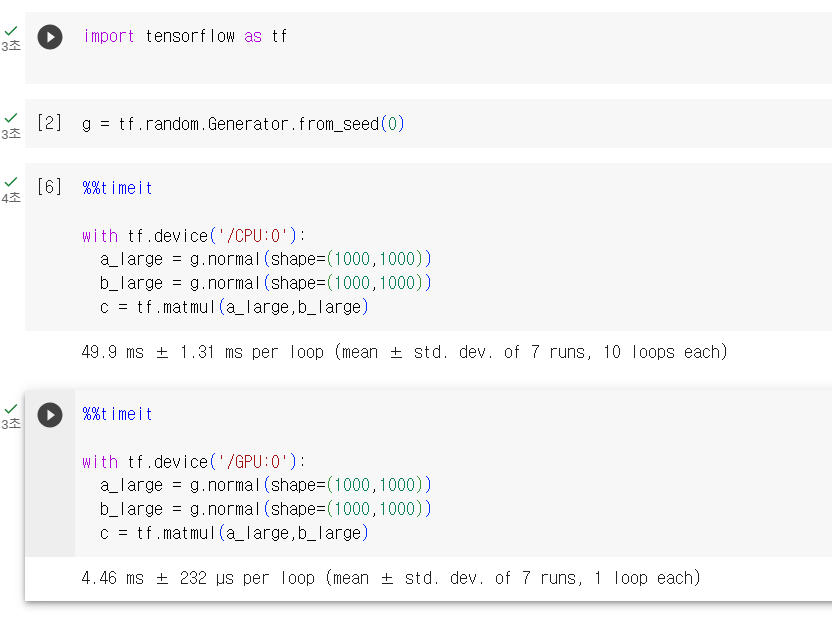
\includegraphics[width=.9\textwidth]{figz/fig1.PNG}
  \caption{행렬곱에서 CPU 와 GPU 의 성능차이: CPU 에서는 루프 당 49.9ms 가 걸렸고,
GPU 에서는 4.46ms 가 걸렸다.}
  \label{fig1}
\end{figure}

\subsection{CUDA 와 스트리밍 다중 프로세서}
GPU 의 대표 회사인 Nvidia 는 미국의 반도체 회사로, GPU 시장 점유율 80\% 안팎으로
예측되고 있다\cite{yonhap2023data}. Nvidia 에서는 GPU 를 GPGPU 로 활용하기 위해 필요한 CUDA 를
개발하였고, GPU 를 병렬 연산에 특화된 수천개의 CUDA 코어로 구성 시켰다.

CUDA(compute Unified Device Architecture)는 GPU 에서 수행하는 알고리즘을 C 
프로그래밍 언어 등으로 개발할 수 있도록 하는 GPGPU 기술이다. CUDA 에서, GPU 에서
실행될 병렬 코드를 커널이라고 부르고, 스레드는 이 커널 함수 중의 한 인스턴스이다.
스레드는 블록으로 묶어지며 이 블록이 스트리밍 다중 프로세서 중 한 개에 할당된다.

스트리밍 다중 프로세서(Streaming multiprocessors)는 레지스터 파일, L1 Cache, CUDA코어,
SFU(Special Functional Units), 이중 왑 스케줄러(Dual warp scheduler) 등으로 구성되어 있다.
SFU 는 코사인,사인, 제곱근과 같은 초월 연산을 수행한다. 이중 왑 스케줄러는 할당받은
블록을 왑(warp, 순차적인 ID 를 가지는 스레드 여러 개를 묶음)으로 나누어 CUDA 코어,
SFU 에 할당한다. CUDA 코어는 Fermi 아키텍처를 기준으로, 두 개의 분리된 파이프라인을
가지고 있다. 하나는 32 비트,64 비트 그리고 그 이상의 정수와 논리/비트 별 연산을 위한 INT 
unit 이고, 다른 하나는 단일 정밀도(single-precision) 부동소수점 연산을 할 수 있는 FP 
unit 이다\cite{william2018comsys}.

그리고 Volta 아키텍처부터 텐서 코어라는 것이 추가되었다. 텐서코어는 AI 에 필요한
행렬 연산에 특화된 부동소수점 연산 장치이다. 텐서 코어는 한 사이클에 4x4 행렬을 한번
곱하고 한번 더하는 연산, 정확히는, 16bit 부동소수점 행렬 2 개를 곱하고, 32bit 부동소수점
행렬 하나를 더하는 연산을 여러 번(2017 년 기준으로 64 번) 할 수 있다. 텐서 코어는 쿠다
코어에 비해 512x512 matrix GEMM(행렬을 한번 곱하고 더하는 연산\cite{nvidia2023matrix})연산 기준으로
약 4 배, 4096x 4096 GEMM 연산 기준으로 약 9 배 더 많은 성능을 제공한다\cite{nvidia2017tensor}. 그러나
실제로 딥러닝에서 활용할 때는, 텐서 코어에 적합하게 데이터를 바꾸는 오버헤드로 인해,
실제 성능 향상은 그보다 낮다고 한다\cite{park2020gpu}.

스트리밍 다중 프로세서 여러 개(아키텍처마다 다르다 Nvidia 의 Fermi 의 경우
16 개이다)와 L2 cache, Giga thread(블록을 스트리밍 다중 프로세서에 할당한다)등이 모여
GPU 를 구성하게 된다.

\section{이번 벤치마크에 쓰이는 인공지능 모델}
\subsection{오픈소스 기반의 그림 인공지능, Stable Diffusion}
오픈소스 기반의 그림 인공지능 중 하나인 Stable Diffusion\cite{rombach2022highresolution}는 독일 뮌헨 대학교에서
개발한 것으로, 개발 비용이 60 만달러정도였다고 예상됨에도\cite{matthias2022training} 2022 년 8 월
22 일오픈소스로 공개하였다\cite{stability2022stable}. 오픈 소스로 공개하여 로컬 컴퓨터에서 실행할 수 있으며,
Stable Diffusion 을 기반으로 한 많은 서비스가 생겼다. Stable Diffusion 을 기반으로 하는
서비스는 Novel AI 등이 있다.

Stable diffusion 은 CLIP\cite{radford2021learning}, U-Net, VAE(Variational Auto Encoder) 등 3 가지 인공신경망으로
구성되어 있다. VAE 인코더는 이미지를 픽셀 공간에서 latent space(이미지를 N 가지 특성에
따라 분류한 것, 512x512 이미지의 경우 $4\times 64\times 64$ 의 latent space 를 가진다)로 압축한다. 이때
노이즈가 추가된다.

CLIP 은 OpenAI 사에서 개발한 이미지와 텍스트 모두를 처리할 수 있는 모델이며 입력된
텍스트와 이미지를 인코딩을 통해 벡터로 변환하고 이 둘을 비교하여 유사도를 측정,
따라서 이미지 인식에 많이 쓰인다. CLIP 은 자연어를 입력하면 $77\times 768$ 의 숫자 값 목록이
생성된다. 이 목록이 U-Net 에 들어가면 이 값을 기반으로 특정 step 수에 도달할 때 까지
random latent space(text-to-image 의 경우), 입력된 이미지에 약간의 noise 가 추가된 latent 
space(image-to-image 의 경우)에서 노이즈를 반복적으로 제거하고 이것을 VAE 디코더가
픽셀 공간으로 변환하여 최종 이미지를 생성한다 U-Net 에는 8 억 6 천만 개의 파라미터가
있고, CLIP 에는 1 억 2 천 3 백만 개의 파라미터가 있다.

Stable Diffusion 의 훈련 데이터는 약 50 억개의 이미지 텍스트 쌍으로, 공개적으로 사용
가능한 데이터 세트 LAION-5B 에서 가져온 것으로 알려져 있으며, Pinterest, WordPress, 
Blogspot, DeviantArt, Wikimedia Commons 등에 있는 이미지로 구성되어 있다\cite{wiki:Stable_Diffusion}.
Stable Diffusion 의 기능은 텍스트를 이미지로 생성하는 기능과 이미지 수정 기능이 있다.

텍스트를 이미지로 생성하는 기능은 텍스트를 입력하면 이미지를 출력하는 기능이고
이미지 수정 기능은, 이미지의 해상도를 올리거나, 그림의 화풍을 바꿀 수 있다. 이런 기능을
사용할 때 이미지 생성에 영향을 주는 시드 값과 추론 단계 수(step)을 조정할 수 있다. 시드
값은 random noise 에 사용되며, 따라서 같은 seed 는 같은 random noise 를 발생시키고, 이는
같은 프롬프트에 대해 같은 이미지를 생성한다. 

추론 단계수는 noise 를 제거하는 단계 수이며, 높이면 더 많은 시간이 들고 너무 낮으면
원하는 이미지가 나오지 않을 수 있다. 또한 Stable diffusion 을 오프라인에서 브라우저를
이용하여 실행할 수 있는 Stable Diffusion WebUI 의 경우 Negative prompt 를 이용해 빼고
싶은 특성을 입력할 수도 있고, Batch size 를 통해 한번에 생성할 이미지 개수를 조정할 수
있다.
\subsection{오픈 소스 기반의 거대 언어 모델, LLaMA}
오픈 소스 기반의 거대 언어 모델은 LLaMA가 있다. LLaMA는 Meta의 오픈소스 언어모델로서 기사, 시, 이야기, 여러 질문에 대한 답변, 소스코드 등을 생성할 수 있다. 현재 LLaMA-1\cite{touvron2023llama}과 LLaMA-2\cite{touvron2023llama2} 가 공개되어 있다. LLaMA-1은 파라미터가 7B, 13B, 33B, 66B개 등을 가진 모델이 있고, LLaMA-2는 7B, 13B, 70B개의 파라미터를 가진 모델이 있다. 또한 각각 4bit양자화 모드와 8bit 양자화 모드가 있는데, 이는 모델의 파라미터를 32bit 부동소수점에서 4bit/8bit 정수로 양자화하여 계산과 메모리 access 속도를 높이는 기법이다. 이 역시 로컬에서 돌릴 수 있다\cite{raghuraman2020introduction}.

LLaMA 훈련에 사용된 데이터셋은 CommonCrawl로 스크랩한 웹페이지, GitHub에 저장되어 있는 소스코드, 20개 언어의 Wikipedia, Project Gutenberg에 업로드된 책, Stack Exchange에 올라와 있는 질문과 답변, ArXiv에 있는 논문의 LaTeX 코드 등이다.

\section{조사범위와 조사방법}
\subsection{조사범위}
현재 출시되고 있는 Nvidia GPU, 즉 RTX 40 series와 RTX 30 series 중 Stable diffusion 벤치마크는 RTX 4090, RTX 4080, RTX 4070Ti, RTX 3090Ti, RTX 3090, RTX 3080Ti, RTX 3080 12GB, RTX 3080, RTX 3070Ti, RTX 3070, RTX 3060Ti, RTX 3060, RTX 3050 이며 LLaMA 벤치마크는 RTX 4090, RTX 4080, RTX 4070Ti, RTX 3090Ti, RTX 3090, RTX 3080Ti, RTX 3080 12GB, RTX 3080, RTX 3060이다.

\subsection{조사 방법}
Stable diffusion 벤치마크 데이터는 아래를 참고하였다.

\href{https://www.tomshardware.com/news/stable-diffusion-gpu-benchmarks}{https://www.tomshardware.com/news/stable-diffusion-gpu-benchmarks}

LLaMA 벤치마크 데이터는 아래를 참고하였다.

\href{https://www.tomshardware.com/news/running-your-own-chatbot-on-a-single-gpu}{https://www.tomshardware.com/news/running-your-own-chatbot-on-a-single-gpu}
\section{GPU 성능비교}
\subsection{GPU별 Stable Diffusion 성능}
아래 \tableautorefname{\ref{stablegpubenchmarktable}}\cite{jarred2023stable}은 $512\times 512$ 이미지를 100 단계로 생성하는 것을 10 번 실행한 것의
iteration per second 의 평균값이다. 이미지 생성을 가속화해주는 Xformers\cite{xFormers2022}를 사용한
결과이다.

% Please add the following required packages to your document preamble:
% \usepackage{graphicx}
\begin{table}[]
\resizebox{\columnwidth}{!}{%
\begin{tabular}{|l|r|r|r|r|}
\hline
GPU           & \multicolumn{1}{l|}{Iteration/sec} & \multicolumn{1}{l|}{가격(US Dollar)} & \multicolumn{1}{l|}{\begin{tabular}[c]{@{}l@{}}가격당 성능(Iteration/sec/USDollar)\\   (소수점 5째자리에서 반올림)\end{tabular}} & \multicolumn{1}{l|}{\begin{tabular}[c]{@{}l@{}}RTX 3060 대비Iteration/sec\\   (단위:배, 3째자리에서 반올림)\end{tabular}} \\ \hline
RTX 4090      & 28.923                             & 1599                               & 0.0181                                                                                                               & 4                                                                                                                \\ \hline
RTX 4080      & 23.504                             & 1199                               & 0.0196                                                                                                               & 3.25                                                                                                             \\ \hline
RTX 4070Ti    & 20.697                             & 799                                & 0.0259                                                                                                               & 2.86                                                                                                             \\ \hline
RTX 3090 Ti   & 19.238                             & 1999                               & 0.0096                                                                                                               & 2.66                                                                                                             \\ \hline
RTX 3090      & 17.789                             & 1499                               & 0.0119                                                                                                               & 2.46                                                                                                             \\ \hline
RTX 3080 Ti   & 17.429                             & 1199                               & 0.0145                                                                                                               & 2.41                                                                                                             \\ \hline
RTX 3080 12GB & 14.459                             & 799                                & 0.0181                                                                                                               & 2                                                                                                                \\ \hline
RTX 3080      & 14.101                             & 699                                & 0.0202                                                                                                               & 1.95                                                                                                             \\ \hline
RTX 3070 Ti   & 11.637                             & 599                                & 0.0194                                                                                                               & 1.61                                                                                                             \\ \hline
RTX 3070      & 10.937                             & 499                                & 0.0219                                                                                                               & 1.51                                                                                                             \\ \hline
RTX 3060 Ti   & 9.146                              & 399                                & 0.0229                                                                                                               & 1.26                                                                                                             \\ \hline
RTX 3060      & 7.239                              & 329                                & 0.0220                                                                                                               & 1                                                                                                                \\ \hline
RTX 3050      & 4.931                              & 249                                & 0.0198                                                                                                               & 0.68                                                                                                             \\ \hline
\end{tabular}%
}
\caption{\label{stablegpubenchmarktable}GPU별 Stable diffusion Iteration per Second for image generation.}
\end{table}

\tableautorefname{\ref{stablegpubenchmarktable}}에서 알 수 있듯, image generation에서 RTX 4090이 28.923 iteration/sec로 가장 높고, RTX 3050이 4.931 iteration/sec로 가장 낮다. 또한 가격당 성능은 RTX 4070Ti가 0.0259로 가장 높고, RTX 3090Ti가 0.0096으로 가장 낮다. 또한 RTX 4090은 RTX 3060 대비 4배 더 높은 초당 Iteration을 생성함을 알 수 있다.

아래 \tableautorefname{\ref{stableresolutiongpubenchmarktable}}\cite{jarred2023stable}는 $768\times 432$ 이미지를 $2048\times 1152$ 의 이미지로 25 단계로 거쳐
바꾸는 것(Image resolution)을 3 개 생성하였을 때 iteration per second 의 값이다. 이미지
생성을 가속화해주는 Xformers\cite{xFormers2022}를 사용한 결과이다.

% Please add the following required packages to your document preamble:
% \usepackage{graphicx}
\begin{table}[]
\resizebox{\columnwidth}{!}{%
\begin{tabular}{|l|r|r|r|r|}
\hline
GPU           & \multicolumn{1}{l|}{Iteration/sec} & \multicolumn{1}{l|}{가격(US Dollar)} & \multicolumn{1}{l|}{\begin{tabular}[c]{@{}l@{}}가격당 성능(Iteration/sec/US Dollar)\\ (소수점 7째자리에서 반올림)\end{tabular}} & \multicolumn{1}{l|}{\begin{tabular}[c]{@{}l@{}}RTX 3060 대비 Iteration/sec \\ (단위: 배, 3째자리에서 반올림)\end{tabular}} \\ \hline
RTX 4090      & 3.641                              & 1599                               & 0.002277                                                                                                        & 7.13                                                                                                          \\ \hline
RTX 4080      & 2.413                              & 1199                               & 0.002013                                                                                                        & 4.72                                                                                                          \\ \hline
RTX 4070Ti    & 1.875                              & 799                                & 0.002347                                                                                                        & 3.67                                                                                                          \\ \hline
RTX 3090 Ti   & 1.558                              & 1999                               & 0.000779                                                                                                        & 3.05                                                                                                          \\ \hline
RTX 3090      & 1.423                              & 1499                               & 0.000949                                                                                                        & 2.78                                                                                                          \\ \hline
RTX 3080 Ti   & 1.358                              & 1199                               & 0.001133                                                                                                        & 2.66                                                                                                          \\ \hline
RTX 3080 12GB & 1.296                              & 799                                & 0.001622                                                                                                        & 2.54                                                                                                          \\ \hline
RTX 3080      & 1.169                              & 699                                & 0.001672                                                                                                        & 2.29                                                                                                          \\ \hline
RTX 3070 Ti   & 0.898                              & 599                                & 0.001499                                                                                                        & 1.76                                                                                                          \\ \hline
RTX 3070      & 0.774                              & 499                                & 0.001551                                                                                                        & 1.51                                                                                                          \\ \hline
RTX 3060 Ti   & 0.674                              & 399                                & 0.001689                                                                                                        & 1.32                                                                                                          \\ \hline
RTX 3060      & 0.511                              & 329                                & 0.001553                                                                                                        & 1                                                                                                             \\ \hline
RTX 3050      & 0.322                              & 249                                & 0.001293                                                                                                        & 0.63                                                                                                          \\ \hline
\end{tabular}%
}
\caption{\label{stableresolutiongpubenchmarktable}GPU별 Stable diffusion Iteration per Second for image resolution.}
\end{table}

\tableautorefname{\ref{stableresolutiongpubenchmarktable}}에서 알 수 있듯, image resolution에서 RTX 4090이 3.641로 가장 높고 RTX 3050이 0.322로 가장 낮다. 가격당 성능은RTX 4070Ti가 0.002347로 가장 높고 RTX 3090Ti가 0.000779로 가장 낮다. 또한 RTX 3060 대비 RTX 4090이 7.13배 더 높은 초당 iteration을 생성함을 알 수 있다.

\subsection{GPU 별 LLaMA성능}
아래 \tableautorefname{\ref{llamabenchmarktable}}\cite{jarred2023howtorun}는 LLaMA-13b 4-bit mode를 Text Generation Web UI라는 LLaMA를 쉽게 오프라인에서 브라우저로 실행할 수 있는 환경에서 실행하여 400개 이상의 토큰을 생성했을 때 초당 token생성 개수이다. 아래 벤치마크를 실행한 환경은 Intel Core i9-12900K(CPU), MSI Pro Z690-A WiFi DDR4(Motherboard), Corsair 2x16GB DDR4-3600 CL16(Main Memory), Crucial P5 Plus 2TB(SSD), Windows 11 Pro 64bit(OS) 등이다.

% Please add the following required packages to your document preamble:
% \usepackage{graphicx}
\begin{table}[]
\resizebox{\columnwidth}{!}{%
\begin{tabular}{|l|r|r|r|r|}
\hline
GPU           & \multicolumn{1}{l|}{Tokens/sec} & \multicolumn{1}{l|}{가격(US Dollar)} & \multicolumn{1}{l|}{\begin{tabular}[c]{@{}l@{}}가격당 성능(Tokens/sec/USDollar) \\ (소수점 5째자리에서 반올림)\end{tabular}} & \multicolumn{1}{l|}{\begin{tabular}[c]{@{}l@{}}RTX 3060 대비 Tokens/sec \\ (단위: 배, 3째자리에서 반올림)\end{tabular}} \\ \hline
RTX 4090      & 25.82                           & 1599                               & 0.0161                                                                                                       & 1.33                                                                                                       \\ \hline
RTX 4080      & 25.44                           & 1199                               & 0.0212                                                                                                       & 1.31                                                                                                       \\ \hline
RTX 4070Ti    & 25.34                           & 799                                & 0.0317                                                                                                       & 1.3                                                                                                        \\ \hline
RTX 3090Ti    & 21.48                           & 1999                               & 0.0107                                                                                                       & 1.1                                                                                                        \\ \hline
RTX 3090      & 20.88                           & 1499                               & 0.0139                                                                                                       & 1.07                                                                                                       \\ \hline
RTX 3080Ti    & 20.73                           & 1199                               & 0.0173                                                                                                       & 1.06                                                                                                       \\ \hline
RTX 3080 12GB & 20.48                           & 799                                & 0.0256                                                                                                       & 1.05                                                                                                       \\ \hline
RTX 3080      & 19.8                            & 699                                & 0.0283                                                                                                       & 1.02                                                                                                       \\ \hline
RTX 3060      & 19.48                           & 329                                & 0.0592                                                                                                       & 1                                                                                                          \\ \hline
\end{tabular}%
}
\caption{\label{llamabenchmarktable}GPU별 Generated Tokens per sec by LLaMA-13B.}
\end{table}

\tableautorefname{\ref{llamabenchmarktable}}에서 알 수 있듯, LLaMA를 실행하여 Tokens/sec을 측정하였을 때RTX 4090이 25.82로 가장 높고, RTX 3060이 19.48로 가장 낮다. 가격당 성능은 RTX 3060이 0.0592로 가장 높고, RTX 3090Ti가 0.0107로 가장 낮다. RTX 4090은 RTX 3060대비 1.33배 더 높은 초당 토큰 수를 보여주었다.
\section{결론}
% Please add the following required packages to your document preamble:
% \usepackage{graphicx}
\begin{table}[]
\resizebox{\columnwidth}{!}{%
\begin{tabular}{|l|r|r|r|r|}
\hline
GPU           & \multicolumn{1}{l|}{\begin{tabular}[c]{@{}l@{}}LLaMA에서\\ RTX 3060 대비 Tokens/sec\\ (단위: 배, 3째자리에서 반올림)\end{tabular}} & \multicolumn{1}{l|}{\begin{tabular}[c]{@{}l@{}}Stable Diffusion image resolution에서\\ RTX 3060 대비 Iteration/sec\\ (단위: 배, 3째자리에서 반올림)\end{tabular}} & \multicolumn{1}{l|}{\begin{tabular}[c]{@{}l@{}}Stable diffusion image generation에서  \\ RTX 3060 대비Iteration/sec \\ (단위:배, 3째자리에서 반올림)\end{tabular}} & \multicolumn{1}{l|}{가격(US Dollar)} \\ \hline
RTX 4090      & 1.33                                                                                                                & 7.13                                                                                                                                               & 4                                                                                                                                                   & 1599                               \\ \hline
RTX 4080      & 1.31                                                                                                                & 4.72                                                                                                                                               & 3.25                                                                                                                                                & 1199                               \\ \hline
RTX 4070Ti    & 1.3                                                                                                                 & 3.67                                                                                                                                               & 2.86                                                                                                                                                & 799                                \\ \hline
RTX 3090Ti    & 1.1                                                                                                                 & 3.05                                                                                                                                               & 2.66                                                                                                                                                & 1999                               \\ \hline
RTX 3090      & 1.07                                                                                                                & 2.78                                                                                                                                               & 2.46                                                                                                                                                & 1499                               \\ \hline
RTX 3080Ti    & 1.06                                                                                                                & 2.66                                                                                                                                               & 2.41                                                                                                                                                & 1199                               \\ \hline
RTX 3080 12GB & 1.05                                                                                                                & 2.54                                                                                                                                               & 2                                                                                                                                                   & 799                                \\ \hline
RTX 3080      & 1.02                                                                                                                & 2.29                                                                                                                                               & 1.95                                                                                                                                                & 699                                \\ \hline
RTX 3060      & 1                                                                                                                   & 1                                                                                                                                                  & 1                                                                                                                                                   & 329                                \\ \hline
\end{tabular}%
}
\caption{\label{conclusiontable}GPU별 AI 성능 비교(RTX 3060 대비).}
\end{table}
본 서베이에서 그림 인공지능과 거대언어모델 실행 용도의 일반 소비자용 Nvidia GPU를 비교하였다. GPU는 부동소수점 연산과 행렬연산에 특화된 반도체로, CPU에 비해 더 빠른 부동소수점연산과 행렬연산을 보여주고 이는 모델을 학습하고 실행하는데도 더 빠르다.     

최근 많은 웹서버 기반의 그림 인공지능과 거대언어모델이 나와 GPU없이도 쉽게 사용할 수 있다. 그러나 이는 개인정보유출 등의 위험이 있고, 회사 등에서는 로컬에서 돌릴 필요가 있다. 최근 오픈소스 기반의 그림 인공지능인 Stable Diffusion과 거대언어모델인 LLaMA가 등장하였으며 GPU만 있으면 로컬에서 돌릴 수 있다. \ref{conclusiontable}를 보면
두 모델 다 RTX 4090이 제일 성능이 좋게 나왔으며Stable diffusion에서는 RTX 3060 대비 RTX 4090의 성능이 적게는 약 4배, 많게는 7배 더 많이 나왔다. 그러나 LLaMA-13B 는 RTX 4090의 성능이 RTX 3060의 성능보다 약 1.33배 빠른 것에 그쳤다.

 RTX 30series(Geforce 30 series)과 RTX 40series (Geforce 40 series)의 모든 GPU를 비교한 것이 아니라 본 서베이에서 비교대상에서 제외된 GPU는 성능을 확인하는데 어려움이 있을 수 있다. 또한 이 결과가 다른 모델(예를 들어, LLaMA-70B)에는 적용되지 않을 수 있다. 또한 LLaMA의 경우 양자화 방법(8bit, GGML, GPTQ)에 따라 다른 성능이 나올 수 있다. 
 
그러나 Stable diffusion의 경우에는 RTX 3060 대비 가격 향상 폭 대비 성능 향상폭이 커서 RTX 4090 그래픽 카드가 필요할 수도 있지만, LLaMA-13b 4bit의 경우 RTX 3060에서 실행해도 RTX 4090에 비해 크게 성능 하락이 없다. 따라서 LLaMA-13b 4bit의 경우 RTX 3060을 사용하여도 크게 문제는 없다.


\bibliographystyle{IEEEtran}
\bibliography{references}

\end{document}